\حصہ{غیر مناسب تکمل}
اب تک قطعی تکمل پر ہم دو شرائط لاگو کرتے آ رہے ہیں۔ پہلی شرط میں تکمل کا دائرہ کار \عددی{a} تا \عددی{b} کا متناہی ہونا لازمی تھا۔ دوسری شرط میں متکمل کا سعت متناہی ہونا ضروری تھا۔ حقیقت میں ہمیں عموماً ایسی صورت سے واسطہ پڑتا ہے جہاں ان میں سے ایک شرط یا دونوں شرائط  مطمئن نہ ہوتے ہوں۔ زیر منحنی \عددی{y=\tfrac{\ln x}{x^2}} وقفہ \عددی{x=1} تا \عددی{x=\infty} رقبہ، لامتناہی دائرہ کار کی مثال ہے (شکل \حوالہ{شکل_طریقہ_کیا_رقبہ_متناہی}-الف)۔ اسی طرح زیر منحنی \عددی{y=\tfrac{1}{\sqrt{x}}}  وقفہ \عددی{x=0} تا \عددی{x=1} رقبہ، لامتناہی سعت کی مثال ہے (شکل \حوالہ{شکل_طریقہ_کیا_رقبہ_متناہی}-ب)۔ ہم دونوں مثالوں پر ایک ہی طرح  غور کرتے ہیں۔ ہم پوچھتے  ہیں کہ دائرہ کار ذرہ کم کرنے سے تکمل کتنا ہو گا اور اس کے بعد دائرہ کار کو لامتناہی تک پہنچاتے ہوئے تکمل کا حد تلاش کرتے ہیں۔ اسی طرح ہم متکمل کو متناہی رکھتے ہوئے تکمل دریافت کر کے متکمل کو لامتناہی تک پہنچاتے ہوئے تکمل کا حد تلاش کرتے ہیں۔
\begin{figure}
\centering
\begin{subfigure}{0.45\textwidth}
\centering
\begin{tikzpicture}[font=\small,declare function={f(\x)=ln(\x)/(\x^2);}]
\begin{axis}[small, axis lines=middle,xlabel={$x$},ylabel={$y$},xlabel style={at={(current axis.right of origin)},anchor=west},ylabel style={at={(current axis.above origin)},anchor=south},xtick={1,2,3,4,5,6},ytick={0.1,0.2},xmin=0,enlargelimits=true,axis on top]
\addplot[name path=fun,smooth,domain=1:7]{f(x)}node[pos=0.5,right,yshift=1ex]{$y=\frac{\ln x}{x^2}$};
\path[name path=xaxis](1,0)--(7,0);
\addplot[lgray] fill between[of=xaxis and fun];
\end{axis}
\end{tikzpicture}
\caption{}
\end{subfigure}\hfill
\begin{subfigure}{0.45\textwidth}
\centering
\begin{tikzpicture}[font=\small,declare function={f(\x)=1/sqrt(\x);}]
\begin{axis}[small, axis lines=middle,xlabel={$x$},ylabel={$y$},xlabel style={at={(current axis.right of origin)},anchor=west},ylabel style={at={(current axis.above origin)},anchor=south},xtick={1},ytick={1},enlargelimits=true,axis on top]
\addplot[name path=fun,smooth,domain=0.5:1]{f(x)}node[pos=0.5,right,yshift=1ex]{$y=\frac{1}{\sqrt{x}}$};
\draw(1,0)--(1,{f(1)});
\path[name path=xaxis](0.5,0)--(1,0);
\addplot[lgray] fill between[of=xaxis and fun];
\path[name path=kt](0,{f(0.5)})--(0.5,{f(0.5)});
\path[name path=kb](0,0)--(0.5,0);
\addplot[lgray] fill between[of=kt and kb];
\end{axis}
\end{tikzpicture}
\caption{}
\end{subfigure}
\caption{کیا ان منحنیات کے نیچے رقبے متناہی ہیں؟}
\label{شکل_طریقہ_کیا_رقبہ_متناہی}
\end{figure}
%%%%%%%%%%%%%%%%%%%%%%%
\begin{figure}
\centering
\begin{minipage}{0.45\textwidth}
\centering
\begin{tikzpicture}[font=\small,declare function={f(\x)=ln(\x)/(\x^2);}]
\begin{axis}[small, axis lines=middle,xlabel={$x$},ylabel={$y$},xlabel style={at={(current axis.right of origin)},anchor=west},ylabel style={at={(current axis.above origin)},anchor=south},xtick={1,5},xticklabels={$1$,$b$},ytick={0.1,0.2},xmin=0,enlargelimits=true,axis on top]
\addplot[name path=fun,smooth,domain=1:7]{f(x)}node[pos=0.5,right,yshift=1ex]{$y=\frac{\ln x}{x^2}$};
\addplot[name path=fun,smooth,domain=1:5,draw=none]{f(x)};
\path[name path=xaxis](1,0)--(5,0);
\addplot[lgray] fill between[of=xaxis and fun];
\draw(5,0)--(5,{f(5)});
\end{axis}
\end{tikzpicture}
\caption{زیر منحنی رقبہ (مثال \حوالہ{مثال_طریقہ_حد_رقبہ_الف})}
\label{شکل_مثال_طریقہ_حد_رقبہ_الف}
\end{minipage}\hfill
\begin{minipage}{0.45\textwidth}
\centering
\begin{tikzpicture}[font=\small,declare function={f(\x)=1/sqrt(\x);}]
\begin{axis}[small, axis lines=middle,xlabel={$x$},ylabel={$y$},xlabel style={at={(current axis.right of origin)},anchor=west},ylabel style={at={(current axis.above origin)},anchor=south},xtick={0.6,1},xticklabels={$a$,$1$},ytick={1},enlargelimits=true,axis on top]
\addplot[smooth,domain=0.5:1]{f(x)}node[pos=0.5,right,yshift=1ex]{$y=\frac{1}{\sqrt{x}}$};
\addplot[name path=fun,smooth,domain=0.6:1,draw=none]{f(x)};
\path[name path=xaxis](0.6,0)--(1,0);
\draw(0.6,0)--(0.6,{f(0.6)});
\draw(1,0)--(1,{f(1)});
\addplot[lgray] fill between[of=xaxis and fun];
\end{axis}
\end{tikzpicture}
\caption{زیر منحنی رقبہ (مثال \حوالہ{مثال_طریقہ_حد_رقبہ_ب})}
\label{شکل_مثال_طریقہ_حد_رقبہ_ب}
\end{minipage}
\end{figure}

\ابتدا{مثال}\شناخت{مثال_طریقہ_حد_رقبہ_الف}
کیا \عددی{x=1} تا \عددی{x=\infty} منحنی \عددی{y=\tfrac{\ln x}{x^2}} کے نیچے رقبہ متناہی ہے؟ ایسا ہونے کی صورت میں اس کی قیمت تلاش کریں۔

حل:\quad
ہم \عددی{x=1} تا \عددی{x=b} اس منحنی کے نیچے رقبہ تلاش کر کے \عددی{b\to \infty} کی صورت میں رقبے کی حد تلاش کرتے ہیں۔ اگر حد متناہی ہو، ہم اس کو لامتناہی منحنی کے نیچے رقبہ تصور کرتے ہیں (شکل \حوالہ{شکل_مثال_طریقہ_حد_رقبہ_الف})۔ آئیں \عددی{x=1} تا \عددی{x=b} رقبہ تلاش کریں۔ 
\begin{align*}
\int_1^b\frac{\ln x}{x^2}\dif x&=\left[(\ln x)\big(-\frac{1}{x}\big)\right]_1^b-\int_1^b\big(-\frac{1}{x}\big)\big(\frac{1}{x}\big)\dif x\\
&=-\frac{\ln b}{b}-\big[\frac{1}{x}\big]_1^b\\
&=-\frac{\ln b}{b}-\frac{1}{b}+1
\end{align*}
بالائی حد \عددی{b\to \infty} کرتے ہوئے رقبے کی حد تلاش کرتے ہیں۔
\begin{align*}
\lim_{b\to\infty}\big[-\frac{\ln b}{b}-\frac{1}{b}+1\big]&=-\big[\lim_{b\to \infty}\frac{\ln b}{b}\big]-0+1\\
&=-\big[\lim_{b\to\infty}\frac{1/b}{1}\big]+1=0+1=1&&\text{\RL{قاعدہ لھوپیٹال}}
\end{align*}
یوں تکملی اظہار میں \عددی{x=1} تا \عددی{x=\infty} زیر منحنی رقبہ درج ذیل ہو گا۔
\begin{align*}
\int_1^{\infty}\frac{\ln x}{x^2}\dif x=\lim_{b\to\infty}\int_1^b\frac{\ln x}{x^2}\dif x=1
\end{align*} 
\انتہا{مثال}
%====================
\ابتدا{مثال}\شناخت{مثال_طریقہ_حد_رقبہ_ب}
کیا \عددی{x=0} تا \عددی{x=1} زیر منحنی \عددی{y=\tfrac{1}{\sqrt{x}}} رقبہ متناہی ہے؟ اگر ایسا ہو تب رقبہ کتنا ہو گا؟

حل:\quad
ہم \عددی{x=a} تا \عددی{x=1} رقبہ تلاش کر کے \عددی{a\to 0^+} کی صورت میں رقبے کی حد پر نظر ڈالتے ہیں۔ اگر یہ حد متناہی ہو تب ہم اس کو \عددی{0} تا \عددی{1} زیر منحنی رقبہ مانتے ہیں (شکل \حوالہ{شکل_مثال_طریقہ_حد_رقبہ_ب})۔
\begin{align*}
\int_a^1\frac{1}{\sqrt{x}}\dif x=\left.2\sqrt{x}\right\vert_a^1=2-2\sqrt{a}
\end{align*}
اب \عددی{a\to 0^+} کرتے ہوئے رقبے کا حد تلاش کرتے ہیں۔
\begin{align*}
\lim_{a\to 0^+}(2-2\sqrt{a})=2-0=2
\end{align*}
یوں تکملی اظہار میں \عددی{0} تا \عددی{1} زیر منحنی رقبہ درج ذیل ہو گا۔
\begin{align*}
\int_0^1\frac{1}{\sqrt{x}}\dif x=\lim_{a\to 0^+}\int_a^1\frac{1}{\sqrt{x}}\dif x=2
\end{align*}
\انتہا{مثال}
%====================

\جزوحصہء{غیر مناسب تکمل}
مثال \حوالہ{مثال_طریقہ_حد_رقبہ_الف} اور مثال \حوالہ{مثال_طریقہ_حد_رقبہ_ب} میں تکمل غیر مناسب ہیں۔

\ابتدا{تعریف}
وہ تکمل جن کے حد لامتناہی ہوں اور وہ تکمل جن کے متکمل وقفہ تکمل کے کسی نقطہ پر لامتناہی قیمت رکھتا ہو \اصطلاح{غیر مناسب تکمل} کہلاتے ہیں۔ اگر تکمل کا حد موجود ہو تب اس حد کو درج ذیل طریقہ سے حاصل کیا جاتا ہے۔
\begin{enumerate}[a.]
\item
اگر وقفہ \عددی{[a,\infty)} پر \عددی{f} استمراری ہو تب درج ذیل ہو گا۔
\begin{align}
\int_a^{\infty}f(x)\dif x=\lim_{b\to\infty}\int_a^bf(x)\dif x
\end{align}
\item
اگر وقفہ \عددی{(-\infty,b]} پر \عددی{f} استمراری ہو تب درج ذیل ہو گا۔
\begin{align}
\int_{-\infty}^bf(x)\dif x=\lim_{a\to-\infty}\int_a^bf(x)\dif x
\end{align}
\item
اگر وقفہ \عددی{(a,b]} پر \عددی{f} استمراری ہو تب درج ذیل ہو گا۔
\begin{align}
\int_a^bf(x)\dif x=\lim_{c\to a^+}\int_c^bf(x)\dif x
\end{align}
\item
اگر وقفہ \عددی{[a,b)} پر \عددی{f} استمراری ہو تب درج ذیل ہو گا۔
\begin{align}
\int_a^bf(x)\dif x=\lim_{c\to b^-}\int_a^cf(x)\dif x
\end{align}
\end{enumerate}
اگر تکمل کا حد متناہی ہو تب ہم کہتے ہیں کہ یہ غیر مناسب تکمل \اصطلاح{مرتکز}\فرہنگ{مرتکز}\فرہنگ{convergent} ہے اور تکمل کے حد کو اس غیر مناسب تکمل کی قیمت تصور کرتے ہیں۔ اگر تکمل کا حد غیر موجود ہو تب ہم کہتے ہیں کہ یہ غیر مناسب تکمل \اصطلاح{منفرج}\فرہنگ{منفرج}\فرہنگ{divergent}  ہے۔
\انتہا{تعریف}
%=====================

تعریف کی پہلی شق مثال \حوالہ{مثال_طریقہ_حد_رقبہ_الف} میں نظر آتی ہے:
\begin{align*}
\int_1^{\infty}\frac{\ln x}{x^2}\dif x&=\lim_{b\to\infty}\int_1^b\frac{\ln x}{x^2}\dif x=1&&\text{\RL{بالائی حد لا متناہی ہے}}
\end{align*}
تعریف کی تیسری شق مثال \حوالہ{مثال_طریقہ_حد_رقبہ_ب} میں نظر آتی ہے:
\begin{align*}
\int_0^1\frac{1}{\sqrt{x}}\dif x&=\lim_{a\to 0^+}\int_a^1\frac{1}{\sqrt{x}}\dif x=2&&\text{\RL{تکمل کے زیریں حد پر متکمل لامتناہی ہے}}
\end{align*}
مذکورہ بالا دونوں صورتوں میں تکمل کا حد متناہی ہے۔ اگلی مثال میں تکمل منفرج ہے۔

\ابتدا{مثال}\شناخت{مثال_طریقہ_منفرج_غیر_مناسب_تکمل}\ترچھا{منفرج غیر مناسب تکمل}\\
درج ذیل تکمل کی مرکوزیت پر غور کریں۔
\begin{align*}
\int_0^1\frac{1}{1-x}\dif x
\end{align*}
حل:\quad
وقفہ \عددی{[0,1)} پر متکمل \عددی{f(x)=\tfrac{1}{1-x}} استمراری ہے  لیکن \عددی{a\to 1^-} کرنے سے یہ لامتناہی ہوتا ہے (شکل \حوالہ{شکل_مثال_طریقہ_منفرج_غیر_مناسب_تکمل})۔ ہم تکمل کی قیمت حاصل کرنے کی کوشش کرتے ہیں۔
\begin{align*}
\lim_{b\to1^-}\int_0^b\frac{1}{1-x}\dif x&=\lim_{b\to 1^-}\big[-\ln\abs{1-x}\big]_0^b\\
&=\lim_{b\to 1^-}[-\ln(1-b)+0]=\infty
\end{align*}
تکمل کا حد لامتناہی ہے لہٰذا یہ منفرج تکمل ہے۔
\انتہا{مثال}
%==================
\begin{figure}
\centering
\begin{minipage}{0.45\textwidth}
\centering
\begin{tikzpicture}[font=\small,declare function={f(\x)=1/(1-\x);}]
\begin{axis}[small, axis lines=middle,xlabel={$x$},ylabel={$y$},xlabel style={at={(current axis.right of origin)},anchor=west},ylabel style={at={(current axis.above origin)},anchor=south},xtick={0.5,1},xticklabels={$b$,$1$},ytick={1},xmin=0,enlargelimits=true,axis on top]
\addplot[smooth,domain=0:0.6]{f(x)}node[pos=0.9,left,yshift=1ex]{$y=\frac{1}{1-x}$};
\addplot[name path=fun,smooth,domain=0:0.5,draw=none]{f(x)};
\path[name path=xaxis](0,0)--(0.5,0);
\addplot[lgray] fill between[of=xaxis and fun];
\draw(0.5,0)--(0.5,{f(0.5)});
\addplot[] plot coordinates {(1,0) (1,{f(0.5)})};
\end{axis}
\end{tikzpicture}
\caption{غیر مناسب منفرج تکمل (مثال \حوالہ{مثال_طریقہ_منفرج_غیر_مناسب_تکمل})}
\label{شکل_مثال_طریقہ_منفرج_غیر_مناسب_تکمل}
\end{minipage}\hfill
\begin{minipage}{0.45\textwidth}
\centering
\begin{tikzpicture}[font=\small,declare function={f(\x)=1/((\x-1)^(2/3)); g(\x)=1/((1-\x)^(2/3));}]
\begin{axis}[small, axis lines=middle,xlabel={$x$},ylabel={$y$},xlabel style={at={(current axis.right of origin)},anchor=west},ylabel style={at={(current axis.above origin)},anchor=south},xtick={0.5,1,1.6,3},xticklabels={$b$,$1$,$c$,$3$},ytick={1},enlargelimits=true,axis on top]
\addplot[smooth,domain=0:0.6]{g(x)};
\addplot[smooth,domain=1.4:3]{f(x)}node[pos=0.25,right,yshift=1ex]{$y=\frac{1}{(x-1)^{2/3}}$};
\addplot[name path=funG,smooth,domain=0:0.5,draw=none]{g(x)};
\path[name path=xaxisG](0,0)--(0.5,0);
\draw(0.5,0)--(0.5,{g(0.5)});
\addplot[lgray] fill between[of=xaxisG and funG];
\addplot[name path=funF,smooth,domain=1.6:3,draw=none]{f(x)};
\path[name path=xaxisF](1.6,0)--(3,0);
\draw(1.6,0)--(1.6,{f(1.6)});
\addplot[lgray] fill between[of=xaxisF and funF];
\addplot[] plot coordinates {(1,0) (1,{f(1.4)})};
\draw(3,0)--(3,{f(3)});
\end{axis}
\end{tikzpicture}
\caption{اندرون نقطہ پر لامتناہی متکمل (مثال \حوالہ{مثال_طریقہ_اندرون_نقطہ_پر_لا_متناہی})}
\label{شکل_مثال_طریقہ_اندرون_نقطہ_پر_لا_متناہی}
\end{minipage}
\end{figure}
%==================
مذکورہ بالا تعریف کو وسعت دیتے ہوئے ان تکمل جن کے زیریں اور بالائی حدود دونوں لامتناہی ہوں پر لاگو کیا جاتا ہے۔ ہم ان پر اسی حصے میں بعد میں غور کریں گے۔ وقفہ تکمل کے اندر نقطہ \عددی{d} پر لامتناہی متکمل کی صورت پر بھی یہ تعریف لاگو کی جاتی ہے۔ ہم ایسے تکمل کو دو ٹکڑوں میں تقسیم کرتے  ہوئے \عددی{a} تا \عددی{b} تکمل کو \عددی{a} تا \عددی{d} تکمل اور \عددی{d} تا \عددی{b} تکمل کا مجموعہ لیتے ہیں۔

\ابتدا{تعریف}
اگر وقفہ \عددی{[a,b]} کے اندرون کسی نقطہ \عددی{d} پر متکمل \عددی{f} کی قیمت لامتناہی ہو تب درج ذیل ہو گا۔
\begin{align}
\int_a^bf(x)\dif x=\int_a^df(x)\dif x+\int_d^bf(x)\dif x
\end{align}
اگر \عددی{a} تا \عددی{d} اور \عددی{d} تا \عددی{b} تکمل مرتکز ہوں تب \عددی{a} تا \عددی{b} تکمل \اصطلاح{مرتکز} ہو گا ورنہ \عددی{a} تا \عددی{b} تکمل \اصطلاح{منفرج} ہو گا۔
\انتہا{تعریف}
%=====================

\ابتدا{مثال}\شناخت{مثال_طریقہ_اندرون_نقطہ_پر_لا_متناہی}\ترچھا{اندرونی نقطہ پر لامتناہی}\\
درج ذیل تکمل کی مرکوزیت پر غور کریں۔
\begin{align*}
\int_0^3\frac{\dif x}{(x-1)^{2/3}}
\end{align*}
حل:\quad
متکمل \عددی{f(x)=\tfrac{1}{(x-1)^{2/3}}} نقطہ \عددی{x=1} پر لامتناہی ہے جبکہ وقفہ \عددی{[0,1)} اور \عددی{(1,3]} پر یہ استمراری ہے (شکل \حوالہ{شکل_مثال_طریقہ_اندرون_نقطہ_پر_لا_متناہی})۔ وقفہ \عددی{[0,3]} پر تکمل کی مرکوزیت وقفہ \عددی{0} تا \عددی{1} اور وقفہ \عددی{1} تا \عددی{3} پر تکمل کی مرکوزیت پر منحصر ہے۔ وقفہ \عددی{[0,1]} پر 
\begin{align*}
\int_0^1\frac{\dif x}{(x-1)^{2/3}}&=\lim_{b\to 1^-}\int_0^b\frac{\dif x}{(x-1)^{2/3}}\\
&=\lim_{b\to 1^-}[3(b-1)^{1/3}-3(0-1)^{1/3}]=3
\end{align*}
اور وقفہ \عددی{[1,3]} پر
\begin{align*}
\int_1^3\frac{\dif x}{(x-1)^{2/3}}&=\lim_{c\to 1^+}\int_c^3\frac{\dif x}{(x-1)^{2/3}}\\
&=\lim_{c\to 1^+}[3(3-1)^{1/3}-3(c-1)^{1/3}]=3\sqrt[3]{2}
\end{align*}
ہو گا۔دونوں حد متناہی ہیں لہٰذا وقفہ \عددی{0} تا \عددی{3} تفاعل \عددی{f} کا تکمل مرتکز ہو گا اور اس کی قیمت \عددی{3+3\sqrt[3]{2}} ہو گی۔
\انتہا{مثال}
%=================
\ابتدا{مثال}\شناخت{مثال_طریقہ_ٹھوس_بگل}
محور \عددی{x} کے عمودی ایک بگل کا رقبہ عمودی تراش دائری قرص ہیں جن کے قطر وقفہ \عددی{-\infty<x\le \ln 2} پر محور \عددی{x} سے  منحنی \عددی{y=e^x} تک ہیں (شکل \حوالہ{شکل_مثال_طریقہ_ٹھوس_بگل})۔ اس بگل کا حجم تلاش کریں۔

حل:\quad
ایک علامتی رقبہ عمودی تراش کا رقبہ
\begin{align*}
S(x)=\pi (\text{\RL{رداس}})^2=\pi\big(\frac{1}{2}y\big)^2=\frac{\pi}{4}e^{2x}
\end{align*}
ہو گا۔ہم \عددی{b\to-\infty} کرتے ہوئے \عددی{b} تا \عددی{\ln 2} تک حجم کی حد کو بگل کا حجم مانتے ہیں۔ ہم حصہ \حوالہ{حصہ_استعمال_تکمل_ترکیب_ٹکیاں} کی طرح ٹکیاں کاٹ کر حجم تلاش کرتے ہیں۔
\begin{align*}
H&=\int_b^{\ln 2}S(x)\dif x=\int_b^{\ln 2}\frac{\pi}{4}e^{2x}\dif x=\left.\frac{\pi}{8}e^{2x}\right\vert_b^{\ln 2}\\
&=\frac{\pi}{8}(e^{\ln 4}-e^{2b})=\frac{\pi}{8}(4-e^{2b})
\end{align*}
اب \عددی{b\to-\infty} کرنے سے \عددی{e^{2b}\to 0} لہٰذا \عددی{H\to \tfrac{\pi}{8}(4-0)=\tfrac{\pi}{2}} ہوتا ہے۔یوں  بگل کا حجم \عددی{\tfrac{\pi}{2}} ہو گا۔ 
\انتہا{مثال}
%======================
\begin{figure}
\centering
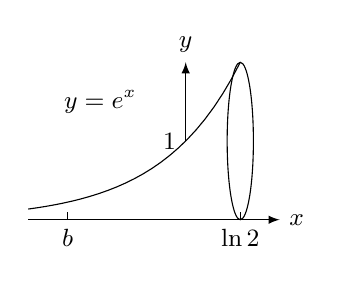
\begin{tikzpicture}[font=\small,declare function={f(\x)=e^(\x);}]
\pgfmathsetmacro{\b}{ln(2)}
\pgfmathsetmacro{\rb}{1/2*f(\b)}
\draw[-latex](-2,0)--(\b+0.5,0)node[right]{$x$};
\draw[-latex](0,{f(0)})node[left]{$1$}--(0,2)node[above]{$y$};
\draw plot [domain=-2:\b]({\x},{f(\x)});
\draw(\b,\rb) circle (1/6*\rb cm and \rb cm);
\draw (-1.5,0)node[below]{$b$}--++(0,0.1)  (\b,0)node[below]{$\ln 2$}--++(0,0.1);
\draw(-0.5,1.5)node[left]{$y=e^x$};
\end{tikzpicture}
\caption{ٹھوس بگل کا حجم (مثال \حوالہ{مثال_طریقہ_ٹھوس_بگل})}
\label{شکل_مثال_طریقہ_ٹھوس_بگل}
\end{figure}

\ابتدا{مثال}
تکمل \عددی{\int_2^{\infty}\tfrac{x+3}{(x-1)(x^2+1)}\dif x} حل کریں۔

حل:
\begin{align*}
\int_2^{\infty}\frac{x+3}{(x-1)(x^2+1)}\dif x&=\lim_{b\to \infty}\int_2^b\frac{x+3}{(x-1)(x^2+1)}\dif x\\
&=\lim_{b\to\infty}\int_2^b\big(\frac{2}{x-1}-\frac{2x+1}{x^2+1}\big)\dif x&&\text{\RL{جزوی کسر}}\\
&=\lim_{b\to\infty}\big[2\ln(x-1)-\ln(x^2+1)-\tan^{-1}x\big]_2^b\\
&=\lim_{b\to\infty}\big[\ln\frac{(x-1)^2}{x^2+1}-\tan^{-1}x\big]_2^b&&\text{\RL{لوگارتھمی اجزاء یکجا}}\\
&=\lim_{b\to \infty}\big[\ln\frac{(b-1)^2}{b^2+1}-\tan^{-1}b\big]-\ln\big(\frac{1}{5}\big)+\tan^{-1}2\\
&=0-\frac{\pi}{2}+\ln 5+\tan^{-1}2\approx 1.1458
\end{align*}
\انتہا{مثال}
%=====================

آپ نے دیکھا کہ \عددی{b\to \infty} کر کے حد کی تلاش سے پہلے ہم نے لوگارتھمی اجزاء کو یکجا کیا۔ اگر ہم ایسا نہ کرتے تب ہمیں درج ذیل نا قابل معلوم مقدار ملتی۔
\begin{align*}
\lim_{b\to \infty} [(2\ln(b-1))-\ln(b^2+1)]=\infty-\infty
\end{align*} 

\جزوحصہء{$-\infty$ سے $\infty$ تک تکمل}
روشنی، بجلی اور  صدا پر غور کرنے سے ایسے تکمل حاصل ہوتے ہیں جن کے دونوں حد لامتناہی ہوتے ہیں۔ اگلا تعریف ان کی مرکوزیت پر ہے۔

\ابتدا{تعریف}
اگر وقفہ \عددی{(-\infty,\infty)} پر \عددی{f} استمراری ہو اور اگر \عددی{\int_{-\infty}^af(x)\dif x} اور \عددی{\int_a^{\infty}f(x)\dif x} دونوں مرتکز ہوں تب ہم کہتے ہیں کہ \عددی{\int_{-\infty}^{\infty}f(x)\dif x} مرتکز ہے اور اس کی قیمت 
\begin{align}\label{مساوات_طریقہ_لامتناہی_حدود_کا_تکمل}
\int_{-\infty}^{\infty}f(x)\dif x=\int_{-\infty}^af(x)\dif x+\int_a^{\infty}f(x)\dif x
\end{align}
مانتے ہیں۔اگر دائیں ہاتھ ایک بھی تکمل منفرج ہو تب \عددی{-\infty} سے \عددی{\infty} تک \عددی{f} کا تکمل منفرج ہو گا۔
\انتہا{تعریف}
%=====================

ہم یہ دکھا سکتے ہیں کہ مساوات \حوالہ{مساوات_طریقہ_لامتناہی_حدود_کا_تکمل} میں \عددی{a} کی قیمت اہمیت نہیں رکھتی ہے۔ ہم \عددی{a} کی کوئی بھی موزوں قیمت لے کر  \عددی{\int_{-\infty}^{\infty}f(x)\dif x} کی مرکوزیت دریافت کر سکتے ہیں۔

تفاعل \عددی{f} کا \عددی{-\infty} سے \عددی{\infty} تک تکمل \عددی{\lim_{b\to\infty}\int_{-b}^bf(x)\dif x} سے مختلف ہو سکتا ہے، جو \عددی{\int_{-\infty}^{\infty}f(x)\dif x} کی عدم مرکوزیت کی صورت میں بھی موجود ہو سکتا ہے۔

\ابتدا{مثال}\شناخت{مثال_طریقہ_لامتناہی_خطہ_کا_رقبہ_الف}
\begin{align*}
\int_{-\infty}^{\infty}\frac{\dif x}{1+x^2}&=\int_{-\infty}^0\frac{\dif x}{1+x^2}+\int_0^{\infty}\frac{\dif x}{1+x^2}&&\text{\RL{مساوات \حوالہ{مساوات_طریقہ_لامتناہی_حدود_کا_تکمل} میں $a=0$}}\\
&=\lim_{b\to-\infty}[\tan^{-1}x]_b^0+\lim_{c\to\infty}[\tan^{-1}x]_0^c\\
&=\lim_{b\to-\infty}[\tan^{-1}0-\tan^{-1}b]+\lim_{c\to\infty}[\tan^{-1}c-\tan^{-1}0]\\
&=0-\big(-\frac{\pi}{2}\big)+\frac{\pi}{2}-0=\pi
\end{align*}
ہم محور \عددی{x} اور منحنی \عددی{y=\tfrac{1}{1+x^2}} کے نیچے لامتناہی خطے کے رقبہ کو تکمل کی قیمت مانتے ہیں (شکل \حوالہ{شکل_مثال_طریقہ_لامتناہی_خطہ_کا_رقبہ_الف})۔
\انتہا{مثال}
%====================
\begin{figure}
\centering
\begin{tikzpicture}[font=\small,declare function={f(\x)=1/(1+\x^2);}]
\begin{axis}[small, axis lines=middle,xlabel={$x$},ylabel={$y$},xlabel style={at={(current axis.right of origin)},anchor=west},ylabel style={at={(current axis.above origin)},anchor=south},ytick={1},enlargelimits=true,axis on top]
\addplot[name path=fun,smooth,domain=-3:3]{f(x)}node[pos=0.75,right,yshift=1ex]{$y=\frac{1}{1+x^2}$};
\path[name path=xaxis](-3,0)--(3,0);
\addplot[lgray] fill between[of=xaxis and fun];
\end{axis}
\end{tikzpicture}
\caption{دونوں اطراف لامتناہی منحنی کے نیچے رقبہ متناہی ہے۔}
\label{شکل_مثال_طریقہ_لامتناہی_خطہ_کا_رقبہ_الف}
\end{figure}

\جزوحصہء{تکمل$\int_1^{\infty}\tfrac{\dif x}{x^p}$}
تکمل \عددی{\int_1^{\infty}\tfrac{\dif x}{x^p}} کی مرکوزیت \عددی{p} پر منحصر ہے۔ اگلی مثال میں \عددی{p=1} اور \عددی{p=2} کے لئے اس حقیقت کو دیکھتے ہیں۔

\ابتدا{مثال}\شناخت{مثال_طریقہ_منحنی_کے_نیچے_رقبہ_متناہی_یا_نہیں}
درج ذیل کی مرکوزیت پر غور کریں۔
\begin{align*}
\int_1^{\infty}\frac{\dif x}{x^2} \quad\text{\RL{اور}}\quad  \int_1^{\infty}\frac{\dif x}{x}
\end{align*}
حل:\quad
وقفہ \عددی{[1,\infty)} پر دونوں تفاعل استمراری ہیں اور \عددی{x\to\infty} کرنے سے دونوں کے ترسیم محور \عددی{x} کے قریب آتے ہیں (شکل \حوالہ{شکل_مثال_طریقہ_منحنی_کے_نیچے_رقبہ_متناہی_یا_نہیں}) لہٰذا کیا ہم کہہ سکتے ہیں کہ دونوں منحنیات کے نیچے رقبے متناہی ہوں گے؟ پہلے تکمل کی صورت میں
\begin{align*}
\int_1^{\infty}\frac{\dif x}{x}=\lim_{b\to \infty}\int_1^b\frac{\dif x}{x}=\lim_{b\to \infty}(\ln b-\ln 1)=\infty 
\end{align*}
ہے لہٰذا تکمل منفرج ہو گا۔دوسری تکمل کی صورت میں
\begin{align*}
\int_1^{\infty}\frac{\dif x}{x^2}=\lim_{b\to \infty}\int_1^b \frac{\dif x}{x^2}=\lim_{b\to \infty}\big(-\frac{1}{b}+1\big)=1
\end{align*}
ہے لہٰذا تکمل مرتکز ہے اور اس کی قیمت \عددی{1} ہے۔
\انتہا{مثال}
%============
\begin{figure}
\centering
\begin{subfigure}{0.45\textwidth}
\centering
\begin{tikzpicture}[font=\small,declare function={f(\x)=1/(\x);}]
\begin{axis}[small, axis lines=middle,xlabel={$x$},ylabel={$y$},xlabel style={at={(current axis.right of origin)},anchor=west},ylabel style={at={(current axis.above origin)},anchor=south},xtick={1,3},xticklabels={$1$,$b$},ytick={1},enlargelimits=true,axis on top]
\addplot[smooth,domain=0.5:3.5]{f(x)}node[pos=0.25,right,yshift=2ex]{$y=\frac{1}{x}$};
\addplot[name path=fun,smooth,domain=1:3,draw=none]{f(x)};
\path[name path=xaxis](1,0)--(3,0);
\addplot[lgray] fill between[of=xaxis and fun];
\draw(1,0)--(1,{f(1)})  (3,0)--(3,{f(3)});
\end{axis}
\end{tikzpicture}
\caption{}
\end{subfigure}\hfill
\begin{subfigure}{0.45\textwidth}
\centering
\begin{tikzpicture}[font=\small,declare function={f(\x)=1/(\x^2);}]
\begin{axis}[small, axis lines=middle,xlabel={$x$},ylabel={$y$},xlabel style={at={(current axis.right of origin)},anchor=west},ylabel style={at={(current axis.above origin)},anchor=south},xtick={1,3},xticklabels={$1$,$b$},ytick={1},enlargelimits=true,axis on top]
\addplot[smooth,domain=0.5:3.5]{f(x)}node[pos=0.25,right,yshift=2ex]{$y=\frac{1}{x^2}$};
\addplot[name path=fun,smooth,domain=1:3,draw=none]{f(x)};
\path[name path=xaxis](1,0)--(3,0);
\addplot[lgray] fill between[of=xaxis and fun];
\draw(1,0)--(1,{f(1)})  (3,0)--(3,{f(3)});
\end{axis}
\end{tikzpicture}
\caption{}
\end{subfigure}
\caption{ایک منحنی کے نیچے رقبہ لا متناہی اور دوسرے کے نیچے متناہی ہے (مثال\حوالہ{مثال_طریقہ_منحنی_کے_نیچے_رقبہ_متناہی_یا_نہیں})۔}
\label{شکل_مثال_طریقہ_منحنی_کے_نیچے_رقبہ_متناہی_یا_نہیں}
\end{figure}

 عموماً \عددی{p>1} کی صورت میں \عددی{\int_1^{\infty}\tfrac{\dif x}{x^p}} مرتکز اور \عددی{p\le 1} کی صورت میں منفرج ہو گا۔

\جزوحصہء{ارتکاز اور انفراج کے پرکھ}
جب کسی غیر مناسب تکمل کی قیمت بلا واسطہ قابل حل نہ ہو (جیسا عموماً ہو گا) تب ہم دو اقدام طریقہ استعمال کرتے ہوئے پہلے ارتکاز ثابت کرتے ہیں اور اس کے بعد اعدادی تراکیب سے تکمل کی قیمت دریافت کرتے ہیں۔ ارتکاز کے بنیادی پرکھ دو ہیں: تقابلی پرکھ اور تقابل حد پرکھ ہیں۔

\ابتدا{مثال}\شناخت{مثال_طریقہ_ارتکاز_پرکھ}
تکمل \عددی{\int_1^{\infty}e^{-x^2}\dif x} کے ارتکاز پر غور کریں۔

حل:\quad
تعریف کی رو سے
\begin{align*}
\int_1^{\infty}e^{-x^2}\dif x=\lim_{b\to \infty}\int_1^b e^{-x^2}\dif x
\end{align*}
ہو گا۔ چونکہ یہ تکمل غیر بنیادی ہے لہٰذا اس کو ہم بلا واسطہ حل نہیں کر سکتے ہیں۔ البتہ ہم دکھا سکتے ہیں کہ \عددی{b\to \infty} کرتے ہوئے اس کا حد متناہی ہے۔ہم جانتے ہیں کہ \عددی{\int_1^be^{-x^2}\dif x} متغیر \عددی{b} کا بڑھتا تفاعل ہے لہٰذا \عددی{b\to \infty} کرنے سے یا یہ لامتناہی ہو گا اور یا \عددی{b\to \infty} کرنے سے اس کا حد متناہی ہو گا۔ اب ہر \عددی{ x\ge1} کے لئے \عددی{e^{-x^2}\le e^{-x}} ہے (شکل \حوالہ{شکل_مثال_طریقہ_ارتکاز_پرکھ}) لہٰذا
\begin{align*}
\int_1^be^{-x^2}\dif x\le \int_1^be^{-x}\dif x=e^{-b}+e^{-1}<e^{-1}\approx 0.36788
\end{align*}
ہو گا اور یوں تکمل لامتناہی نہیں ہے۔یوں
\begin{align*}
\int_1^{\infty}e^{-x^2}\dif x=\lim_{b\to\infty}\int_1^be^{-x^2}\dif x
\end{align*}
کسی مخصوص قیمت کو مرتکز ہو گا۔ ہم اس تکمل کی قیمت نہیں جانتے ہیں البتہ اتنا ضرور جانتے ہیں کہ تکمل کی قیمت \عددی{0.37} سے کم ہے۔
\انتہا{مثال}
%======================
\begin{figure}
\centering
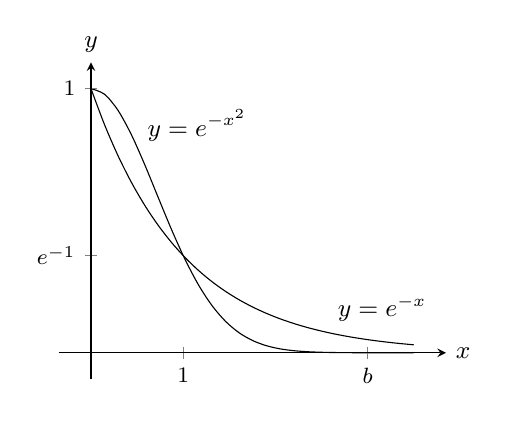
\begin{tikzpicture}[font=\small,declare function={f(\x)=e^(-\x^2);g(\x)=e^(-\x);}]
\pgfmathsetmacro{\k}{e^(-1)}
\begin{axis}[small, axis lines=middle,xlabel={$x$},ylabel={$y$},xlabel style={at={(current axis.right of origin)},anchor=west},ylabel style={at={(current axis.above origin)},anchor=south},xtick={1,3},xticklabels={$1$,$b$},ytick={1,\k},yticklabels={$1$,$e^{-1}$},enlargelimits=true,axis on top]
\addplot[smooth,domain=0:3.5]{f(x)}node[pos=0.15,right,yshift=2ex]{$y=e^{-x^2}$};
\addplot[smooth,domain=0:3.5]{g(x)}node[pos=0.75,right,yshift=2ex]{$y=e^{-x}$};
\end{axis}
\end{tikzpicture}
\caption{وقفہ $x>1$ پر ترسیم $e^{-x^2}$ ترسیم $e^{-x}$ کے نیچے ہے۔}
\label{شکل_مثال_طریقہ_ارتکاز_پرکھ}
\end{figure}

تفاعل \عددی{e^-{x^2}} اور \عددی{e^{-x}} کا پرکھ مثال \حوالہ{مثال_طریقہ_ارتکاز_پرکھ}  میں کیا گیا جو درج ذیل کی ایک مخصوص صورت ہے۔


\ابتدا{مسئلہ}\موٹا{تقابلی پرکھ}\\
فرض کریں وقفہ \عددی{[a,\infty)} پر \عددی{f} اور \عددی{g} استمراری ہیں اور تمام \عددی{x\ge a} پر \عددی{0\le f(x)\le g(x)} ہے۔ تب درج ذیل ہوں  گے۔
\begin{enumerate}[a.]
\item
اگر \عددی{\int_a^{\infty}g(x)\dif x} مرتکز ہو تب \عددی{\int_a^{\infty}f(x)\dif x} مرتکز ہو گا۔
\item
اگر \عددی{\int_a^{\infty}f(x)\dif x} منفرج ہو تب \عددی{\int_a^{\infty}g(x)\dif x} منفرج ہو گا۔
\end{enumerate}
\انتہا{مسئلہ}
%==================

\ابتدا{مثال}
(ا) چونکہ \عددی{[1,\infty)} پر \عددی{0\le \tfrac{\sin^2x}{x^2}\le \tfrac{1}{x^2}} اور  \عددی{\int_1^{\infty}\tfrac{\dif x}{x^2}} مرتکز ہے لہٰذا  \عددی{\int_1^{\infty}\tfrac{\sin^2x}{x^2}\dif x} مرتکز ہو گا۔\\
(ب) چونکہ \عددی{[1,\infty)} پر \عددی{\tfrac{1}{\sqrt{x^2-0.1}}\ge \tfrac{1}{x}} اور  \عددی{\int_1^{\infty}\tfrac{\dif x}{x}} منفرج  ہے لہٰذا  \عددی{\int_1^{\infty}\tfrac{\dif x}{\sqrt{x^2-0.1}}} منفرج ہو گا۔
\انتہا{مثال}
%======================

\ابتدا{مسئلہ}\شناخت{مسئلہ_تراکیب_تکمل_تقابل_حد_پرکھ}\موٹا{تقابل حد پرکھ}\\
اگر \عددی{[a,\infty)} پر مثبت تفاعل \عددی{f} اور \عددی{g} استمراری ہوں اور اگر
\begin{align*}
\lim_{x\to\infty}\frac{f(x)}{g(x)}&=L&&(0<L<\infty)
\end{align*}
ہو تب \عددی{\int_a^{\infty}f(x)\dif x} اور \عددی{\int_a^{\infty}g(x)\dif x} دونوں یا مرتکز ہوں گے اور یا دونوں منفرج ہوں گے۔
\انتہا{مسئلہ}
%============================

حصہ \حوالہ{حصہ_ماورائی_اضافی_شرح_نمو} کی زبان میں مسئلہ \حوالہ{مسئلہ_تراکیب_تکمل_تقابل_حد_پرکھ} کہتا ہے کہ اگر \عددی{x\to\infty} پر  دو تفاعل ایک ہی شرح سے بڑھتے ہوں تب \عددی{a} سے \عددی{\infty} تک ان دونوں کے تکمل کا رویہ ایک دوسرے جیسا ہو گا۔ دونوں مرتکز یا دونوں منفرج ہوں گے۔ اس کا ہرگز یہ مطلب نہیں ہے کہ ان دو تکمل کی قیمت ایک دوسرے جیسی ہو گی۔

\ابتدا{مثال}\شناخت{مثال_طریقہ_رویہ_تفاعل}
درج ذیل کا آپس میں تقابل حد پرکھ کی مدد سے موازنہ کریں۔
\begin{align*}
\int_1^{\infty}\frac{\dif x}{x^2},\quad \int_1^{\infty}\frac{\dif x}{1+x^2}
\end{align*}
حل:\quad
ہم \عددی{f(x)=\tfrac{1}{x^2}} اور \عددی{g(x)=\tfrac{1}{1+x^2}} لیتے ہیں۔ یوں
\begin{align*}
\lim_{x\to\infty}\frac{f(x)}{g(x)}&=\lim_{x\to \infty}\frac{1/x^2}{1/(1+x^2)}\\
&=\lim_{x\to\infty}\frac{1+x^2}{x^2}=\lim_{x\to\infty}\big(\frac{1}{x^2}+1\big)=0+1=1
\end{align*}
متناہی مثبت حد ہے (شکل \حوالہ{شکل_مثال_طریقہ_رویہ_تفاعل})۔ اب چونکہ \عددی{\int_1^{\infty}\tfrac{\dif x}{x^2}} مرتکز ہے لہٰذا \عددی{\int_1^{\infty}\tfrac{\dif x}{1+x^2}} بھی مرتکز ہو گا۔

دونوں تکمل کی قیمتیں البتہ مختلف ہیں۔
\begin{align*}
\int_1^{\infty}\frac{\dif x}{x^2}&=1&&\text{\RL{مثال \حوالہ{مثال_طریقہ_منحنی_کے_نیچے_رقبہ_متناہی_یا_نہیں}}}\\
\int_1^{\infty}\frac{\dif x}{1+x^2}&=\lim_{b\to \infty}\int_1^b\frac{\dif x}{1+x^2}\\
&=\lim_{b\to\infty}[\tan^{-1}b-\tan^{-1}1]=\frac{\pi}{2}-\frac{\pi}{4}=\frac{\pi}{4}
\end{align*}

\انتہا{مثال}
%=================
\begin{figure}
\centering
\begin{tikzpicture}[font=\small,declare function={f(\x)=1/(\x^2); g(\x)=1/(1+\x^2);}]
\begin{axis}[small, axis lines=middle,xlabel={$x$},ylabel={$y$},xlabel style={at={(current axis.right of origin)},anchor=west},ylabel style={at={(current axis.above origin)},anchor=south},xtick={1,2,3},ytick={1},enlargelimits=true,axis on top]
\addplot[smooth,domain=0.9:3]{f(x)}node[pos=0.25,right,yshift=1ex]{$y=\frac{1}{x^2}$};
\addplot[smooth,domain=0:3]{g(x)}node[pos=0.5,below left,yshift=-1ex]{$y=\frac{1}{1+x^2}$};
\end{axis}
\end{tikzpicture}
\caption{تفاعل برائے مثال \حوالہ{مثال_طریقہ_رویہ_تفاعل}}
\label{شکل_مثال_طریقہ_رویہ_تفاعل}
\end{figure}

\ابتدا{مثال}
چونکہ \عددی{\int_1^{\infty}\tfrac{\dif x}{e^x}} مرتکز ہے اور
\begin{align*}
\lim_{x\to\infty}\frac{1/e^x}{3/(e^x+5)}&=\lim_{x\to\infty}\frac{e^x+5}{3e^x}\\
&=\lim_{x\to\infty}\big(\frac{1}{3}+\frac{5}{3e^x}\big)=\frac{1}{3}+0=\frac{1}{3}
\end{align*}
مثبت متناہی حد ہے لہٰذا \عددی{\int_1^{\infty}\tfrac{3}{e^x+5}\dif x} مرتکز ہو گا۔  جہاں تک غیر متناسب تکمل کی ارتکاز کی بات ہے \عددی{\tfrac{3}{e^x+5}} اور \عددی{\tfrac{1}{e^x}} کا رویہ ایک دوسرے جیسا ہے۔ 
\انتہا{مثال}
%=========================

